
\section{Simulado 4}

\num{1}

\begin{quote}
\textbf{Campus Party: reciclagem de lixo eletrônico dá origem a projetos
sociais}

A cada dia surgem novos modelos de computadores, smartphones, câmeras
digitais e outros diversos produtos eletrônicos. A velocidade dos
lançamentos e atualizações faz com que esses equipamentos se tornem
obsoletos rapidamente, e assim cresce a demanda por uma destinação
correta para o lixo eletrônico. Projetos que atuam na reutilização
desses objetos estão sendo apresentados na Campus Party Brasília, que é
realizada até este sábado (17).
\end{quote}

  \fonte{Disponível em:\url{https://agenciabrasil.ebc.com.br/pesquisa-e-inovacao/noticia/2017-06/campus-party-reciclagem-de-lixo-eletronico-da-origem-projetos}.
Acesso em: 08 mar. 2023 (fragmento).}

Da leitura do texto, depreende-se que a grande quantidade gerada de lixo
eletrônico tem como causa

\begin{escolha}
\item a obsolescência dos eletrônicos em razão das rápidas inovações
tecnológicas.

\item o descarte dos equipamentos eletrônicos de forma incorreta no meio
ambiente.

\item a qualidade baixa dos equipamentos eletrônicos que leva a uma curta
vida útil.

\item a falta de projetos sociais que possam dar uma destinação adequada
aos eletrônicos.
\end{escolha}

\num{2}

\begin{quote}
\textbf{Obesidade infantil é tema do programa Salto para o Futuro}

Um dos problemas de saúde pública mais preocupantes atualmente, a
obesidade infantil, será o tema da próxima edição do
programa~\emph{Salto para o Futuro}, nesta quarta-feira, 18, às 20h, na
TV Escola. A escolha da matéria não acontece por acaso, uma vez que a
Organização Mundial de Saúde (OMS), em seu estudo mais recente de
outubro de 2017, apontou um total de 124 milhões de crianças e
adolescentes obesos em todo o mundo.

{[}...{]}

As causas da doença e as medidas para evitar que crianças, adolescentes
e jovens se tornem obesos são o foco desta edição do programa da TV
Escola.
\end{quote}

\fonte{Disponível em:
\url{http://portal.mec.gov.br/ultimas-noticias/33491-tv-escola/63021-obesidade-infantil-e-tema-do-programa-salto-para-o-futuro}.
Acesso em: 08 mar. 2023 (fragmento adaptado).}

No último parágrafo, o termo ``doença'', além de retomar ``obesidade
infantil'', adiciona-lhe um valor semântico. Nesse sentido, o termo
retoma a expressão ``obesidade infantil'' e, ao mesmo tempo,

\begin{escolha}
\item situa-a no horizonte de preocupação da medicina como um problema de
saúde.

\item atenua a gravidade com que se deve observar a obesidade na juventude.

\item relaciona-a aos dados estatísticos da Organização Mundial de Saúde.

\item chama o espectador a acompanhar a edição do programa divulgado.
\end{escolha}

\num{3}

\textbf{TEXTO I}

\begin{quote}
\textbf{Organização e segurança são destaques no carnaval de rua de São
Paulo}

\emph{Prévia de pesquisa entre os foliões de ruas aponta que a
organização teve aprovação de 96,3\% com nota de 8,8, em escala de zero
a dez. Já para o público que esteve no sambódromo, a nota final foi 9
(mais de 50\% deram 10)}
\end{quote}

\fonte{SECRETARIA ESPECIAL DE COMUNICAÇÃO, 23 fev. 2023. Disponível em:
capital.sp.gov.br/noticia/organizacao-e-seguranca-sao-destaques-no-carnaval-de-rua-de-sao-paulo.
Acesso em: 04 mar. 2023.}

\textbf{TEXTO II}

\begin{quote}
\textbf{Mais de 3 mil celulares foram furtados durante o carnaval em SP}

\emph{Número é quase 40\% inferior aos registrados de 2020}

Durante o período de carnaval foram registrados 3.486 roubos e furtos de
celulares no estado de São Paulo, segundo balanço divulgado hoje (22)
pela Secretaria de Segurança Pública de São Paulo.

O número é quase 40\% inferior à quantidade de registros de roubos e
furtos ocorridos no carnaval de 2020, quando foram feitos 5.450 boletins
de ocorrência. O número também é inferior ao que foi registrado no
carnaval de 2019, quando foram lavrados 5.471 boletins.
\end{quote}

\fonte{AGÊNCIA BRASIL, 22 fev. 2023. Disponível em:
\url{https://agenciabrasil.ebc.com.br/geral/noticia/2023-02/mais-de-3-mil-celulares-foram-furtados-durante-o-carnaval-em-sp}.
Acesso em: 04 mar. 2023.}

A aparente divergência entre as informações apresentadas nessas notícias
é afastada

\begin{escolha}
\item pelo conhecimento prévio do leitor.

\item pela presença de dados estatísticos.

\item pela credibilidade dos veículos.

\item pelo meio de circulação.
\end{escolha}

\textbf{Texto para as questões 4 e 5.}

\begin{figure}
\centering
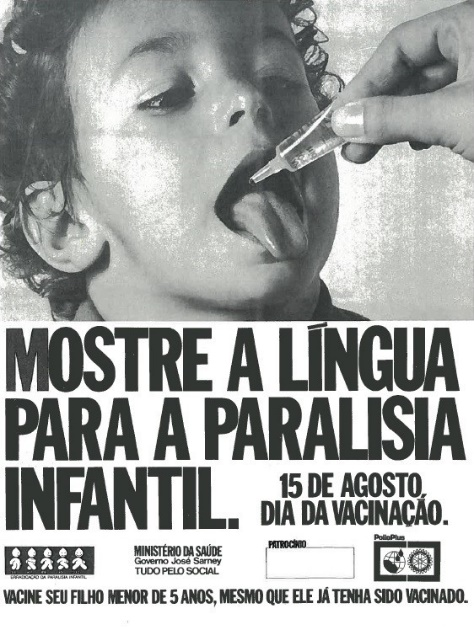
\includegraphics[width=2.12879in,height=2.83333in]{./imgSAEB_8_POR/media/image39.jpeg}
% \caption{Texto Descrição gerada automaticamente}
\end{figure}

\fonte{Disponível em: \url{https://bvsms.saude.gov.br/bvs/folder/10006001944.pdf}.
Acesso em: 09 mar. 2023 (adaptado).}

\num{4}

A campanha, na linguagem verbal e não verbal, busca ganhar a adesão do
público por meio da ênfase

\begin{escolha}
\item na data da vacinação.

\item no motivo da vacinação.

\item no método de vacinação.

\item no público da vacinação.
\end{escolha}


\num{5}

Textos publicitários utilizam diferentes recursos na construção da
mensagem. Na campanha apresentada, o recurso utilizado é

\begin{escolha}
\item
a imparcialidade, para evitar influenciar a adesão do público.
\item
o efeito humorístico, gerado pela pose da criança na fotografia.
\item
a duplicidade de sentidos, como na expressão ``mostre a língua''.
\item
a linguagem literal, privilegiando o sentido denotativo das palavras.
\end{escolha}

\num{6}

\begin{quote}
Passava das 11 horas da noite quando Bento deixou a fazendo do compadre
Chico em sua velha caminhonete vermelha. Estava a pouco menos de vinte
quilômetros de sua casa. Conhecia o caminho como a palma da mão. Os
primeiros cinco quilômetros eram asfaltados. O resto parecia uma
montanha-russa de terra batida, repleta de pedregulhos. Ao passar pela
última porteira, ligou o rádio. Acordara às 6 da manhã e não queria
dormir ao volante. Perdera o melhor amigo em um acidente naquele mesmo
trajeto.
\end{quote}

\fonte{FARAH, F.T. \emph{O enigma das estrelas.} São Paulo: Geração Editorial,
2013 (fragmento).}

Há sentido figurado em

\begin{escolha}
\item ``Os primeiros cinco quilômetros eram asfaltados''.

\item ``O resto parecia uma montanha-russa de terra batida''.

\item ``Estava a pouco menos de vinte quilômetros de sua casa''.

\item ``Perdera o melhor amigo em um acidente naquele mesmo trajeto''.
\end{escolha}


\num{7}

\begin{quote}
Era uma O ônibus Greyhound fez sua parada regular em Meade, Ohio, uma
insignificante cidade produtora de papel a uma hora ao sul de Columbus
que cheirava a ovo podre. Forasteiros

reclamavam do fedor, mas os moradores gostavam de se vangloriar de que
aquele era o doce aroma do dinheiro. O motorista, um homem simplório e
atarracado que usava sapatos com salto e uma gravata borboleta frouxa,
parou no beco ao lado da estação e anunciou uma parada de quarenta
minutos. Desejava poder tomar uma xícara de café, porém sua úlcera
estava atacando novamente. Bocejou e deu um gole numa garrafa de um
remédio rosa que deixava no painel. A chaminé do outro lado da cidade,
de longe a estrutura mais alta naquela parte do estado, arrotava mais
uma nuvem marrom e suja. Era possível vê-la por quilômetros, soprando
como um vulcão prestes a estourar seu topo estreito.
{[}...{]}
\end{quote}

\fonte{POLLOCK, Donald Ray. \emph{O mal nosso de cada dia}. Tradução de Paulo
Raviere. Rio de Janeiro: DarkSide Books, 2020.}

Pelo conteúdo do texto, e sabendo que se trata de uma narrativa, pode-se
reconhecer que esse parágrafo apresenta

\begin{escolha}
\item o desfecho, que introduz a resolução do problema surgido na história.

\item o conflito, que introduz o problema que precisa ser resolvido na
história.

\item a situação inicial, que introduz o tempo, o espaço e os personagens
da história.

\item o clímax, que introduz as tensões entre os personagens e reviravoltas
na história.
\end{escolha}

\textbf{Texto para as questões 8 e 9.}

\begin{quote}
Uma noite destas, vindo da cidade para o Engenho Novo, encontrei no trem
da Central um rapaz aqui do bairro, que eu conheço de vista e de chapéu.
Cumprimentou-me, sentou-se ao pé de mim, falou da Lua e dos ministros, e
acabou recitando-me versos. A viagem era curta, e os versos pode ser que
não fossem inteiramente maus. Sucedeu, porém, que, como eu estava
cansado, fechei os olhos três ou quatro vezes; tanto bastou para que ele
interrompesse a leitura e metesse os versos no bolso.

--- Continue, disse eu acordando.

--- Já acabei, murmurou ele.

--- São muito bonitos.

Vi-lhe fazer um gesto para tirá-los outra vez do bolso, mas não passou
do gesto; estava amuado. No dia seguinte entrou a dizer de mim nomes
feios, e acabou alcunhando-me Dom Casmurro. Os vizinhos, que não gostam
dos meus hábitos reclusos e calados, deram curso à alcunha, que afinal
pegou. Nem por isso me zanguei. Contei a anedota aos amigos da cidade, e
eles, por graça, chamam-me assim, alguns em bilhetes: ``Dom Casmurro,
domingo vou jantar com você''. {[}...{]}
\end{quote}

\fonte{ASSIS, Machado de.~\emph{Dom Casmurro}.~Rio de Janeiro: Nova Aguilar,
1994 (fragmento).}

\num{8}

O narrador considera ser uma anedota a situação que vivenciou com um
rapaz no trem. A situação pode ser considerada engraçada porque

\begin{escolha}
\item a conversa entre o narrador e o rapaz abordou diferentes assuntos.

\item o rapaz interrompeu a leitura e guardou os versos do poema no bolso.

\item o narrador evitou dar atenção ao rapaz por conhecê-lo apenas de
vista.

\item o cansaço do narrador foi confundido com falta de interesse no poema.
\end{escolha}

\num{9}

De acordo com o contexto, o uso da expressão ``fechei os olhos três ou
quatro vezes'' teve o objetivo de

\begin{escolha}
\item diminuir a importância do motivo causador da indignação do rapaz.

\item concordar com o motivo de o rapaz ter desistido da leitura dos
versos.

\item indicar a quantidade de vezes que dormiu ao longo da conversa.

\item justificar sua indiferença em relação ao poema lido pelo rapaz.
\end{escolha}

\num{10}

\begin{quote}
\textbf{O goleiro}

Também chamado de porteiro, guarda-metas, arqueiro, guardião, golquíper
ou guarda-valas, mas poderia muito bem ser chamado de mártir, vítima,
saco de pancadas, eterno penitente ou favorito das bofetadas. Dizem que
onde ele pisa, nunca mais cresce a grama. {[}...{]}

Os outros jogadores podem errar feio uma vez, muitas vezes, mas se
redimem com um drible espetacular, um passe magistral, um tiro certeiro.
Ele, não. A multidão não perdoa o goleiro. Saiu em falso? Catando
borboleta? Deixou a bola escapar? Os dedos de aço se fizeram de seda?
Com uma só falha, o goleiro arruína uma partida ou perde um campeonato,
e então o público esquece subitamente todas as suas façanhas e o condena
à desgraça eterna. Até o fim de seus dias, será perseguido pela
maldição.
\end{quote}

\fonte{GALEANO, Eduardo. \emph{Futebol ao sol e à sombra}. Tradução de Eric
Nepomuceno e Maria do Carmo Brito. Porto Alegre: L\&PM Pocket, 2014
(fragmento).}

O texto aborda a profissão de goleiro com tom humorístico. O efeito de
humor se manifesta por meio de

\begin{escolha}
\item caracterização pejorativa e exagero.

\item uso de termos e expressões ofensivos.

\item desqualificação das habilidades do goleiro.

\item exaltação dos jogadores de linha.
\end{escolha}

\num{11}

\begin{quote}\textbf{Manutenção}

Aumente a vida útil do aparelho, limpe-o regularmente!

NOTA: Antes de iniciar a limpeza do equipamento desligue-o da tomada.

\textbf{Limpando a tela}

\num{1} Molhe um pano macio em uma mistura de água morna com um pouco de
detergente. Esprema bem o pano até que ele fique quase seco e então
utilize-o em sua tela.

\num{2} Para garantir que não exista resíduos líquidos na tela, deixe-a
secar por alguns minutos e só depois ligue o aparelho na tomada.
\end{quote}

\fonte{Disponível em:
\url{https://www.lg.com/br/products/documents/MFL59166617\_BBTV\_SERIES\_REV00.pdf}.
Acesso em: 10 mar. 2023 (fragmento).}

Devido ao gênero a que pertence, o texto apresenta, em sua composição,
verbos no imperativo que expressam o sentido de

\begin{escolha}
\item comando, para que o usuário se sinta obrigado a limpar o equipamento.

\item recomendação, para que o usuário faça a correta limpeza do
equipamento.

\item apelo, para que o usuário reconheça a necessidade de limpar o
equipamento.

\item convite, para que o leitor seja convencido a realizar a limpeza do
equipamento.
\end{escolha}

\num{12}

\textbf{TEXTO I}

\begin{quote}

\textbf{Isto}

Dizem que finjo ou minto

Tudo que escrevo. Não.

Eu simplesmente sinto

Com a imaginação.

Não uso o coração.

Tudo o que sonho ou passo,

O que me falha ou finda,

É como que um terraço

Sobre outra coisa ainda.

Essa coisa é que é linda.

Por isso escrevo em meio

Do que não está ao pé,

Livre do meu enleio,

Sério do que não é.

Sentir? Sinta quem lê!
\end{quote}

\fonte{PESSOA, Fernando. Disponível em:
\url{http://arquivopessoa.net/typographia/textos/arquivopessoa-4250.pdf}.
Acesso em: 10 mar. 2023.}

\textbf{TEXTO II}

\begin{quote}
\textbf{Autopsicografia}

O poeta é um fingidor

Finge tão completamente

Que chega a fingir que é dor

A dor que deveras sente.

E os que leem o que escreve,

Na dor lida sentem bem,

Não as duas que ele teve,

Mas só a que eles não têm.

E assim nas calhas de roda

Gira, a entreter a razão,

Esse comboio de corda

Que se chama coração.
\end{quote}

\fonte{PESSOA, Fernando. Disponível em: \url{http://arquivopessoa.net/textos/4234}. Acesso em: 10 mar. 2023.}

Os dois poemas se relacionam intertextualmente por

\begin{escolha}
\item pertencerem ao mesmo autor.

\item concordarem no mesmo ponto de vista.

\item abordarem o mesmo tema: o fazer poético.

\item apresentarem a mesma estrutura de estrofes.
\end{escolha}

\num{13}

\begin{quote}
\textbf{Como nuvens pelo céu}

Como nuvens pelo céu

Passam os sonhos por mim.

Nenhum dos sonhos é meu

Embora eu os sonhe assim.

São coisas no alto que são

Enquanto a vista as conhece,

Depois são sombras que vão

Pelo campo que arrefece.

Símbolos? Sonhos? Quem torna

Meu coração ao que foi?

Que dor de mim me transtorna?

Que coisa inútil me dói?
\end{quote}

\fonte{PESSOA, Fernando. Disponível em: \url{http://arquivopessoa.net/textos/1063}.
Acesso em: 13 mar. 2023.}

O eu lírico utiliza, em sua reflexão, uma comparação com as nuvens por
sua característica de serem

\begin{escolha}
\item lúdicas.

\item uniformes.

\item transitórias.

\item reconhecíveis.
\end{escolha}

\num{14}

\begin{quote}
Assim como acontece em várias famílias brasileiras, na minha há uma
prática comum: quem ascende socialmente numa capital (no caso, Salvador)
acaba ``puxando'' os parentes do interior. No meu lado paterno, quem
cumpriu esse papel foi Dindinha, tia-avó de meu pai. Ela, aliás, levou
esse costume ao extremo: recebemos nada menos que dezenove sobrinhos na
sua casa, no bairro da Federação.
\end{quote}

\fonte{RAMOS, Lázaro. \emph{Na minha pele}. 1.ed. Rio de Janeiro: Objetiva,
2017 (fragmento).}

Os termos ``esse papel'' e ``esse costume'' contribuem para a progressão
textual ao evitarem repetição de palavras e

\begin{escolha}
\item provocarem mudança de assunto.

\item fazerem referência externa ao texto.

\item anteciparem o que ainda vai ser dito.

\item retomarem o mesmo trecho antecedente.
\end{escolha}

\num{15}

\begin{quote}
Se eu pudesse trincar a terra toda

E sentir-lhe um paladar,

Seria mais feliz um momento...

Mas eu nem sempre quero ser feliz.

É preciso ser de vez em quando infeliz

Para se poder ser natural...

Nem tudo é dias de sol,

E a chuva, quando falta muito, pede-se.

Por isso tomo a infelicidade com a felicidade

Naturalmente, como quem não estranha

Que haja montanhas e planícies

E que haja rochedos e erva...

O que é preciso é ser-se natural e calmo

Na felicidade ou na infelicidade,

Sentir como quem olha,

Pensar como quem anda,

E quando se vai morrer, lembrar-se de que o dia morre,

E que o poente é belo e é bela a noite que fica...

Assim é e assim seja...
\end{quote}

\fonte{PESSOA, Fernando. Disponível em: \url{http://arquivopessoa.net/textos/613}.
Acesso em: 19 mar. 2023.}

O verso final do poema, ``Assim é e assim seja...'', confirma a visão de
mundo exposta ao longo do texto. O eu poético, nesse verso, assume, em
relação aos infortúnios da vida, uma postura de

\begin{escolha}
\item conformismo

\item negação.

\item pessimismo.

\item indignação.
\end{escolha}